\documentclass[tikz,border=6mm]{standalone}
\usepackage{amsmath,amssymb}
\usepackage{fontspec}

\usetikzlibrary{positioning,arrows.meta}

% Pure black-and-white palette for print
\begin{document}
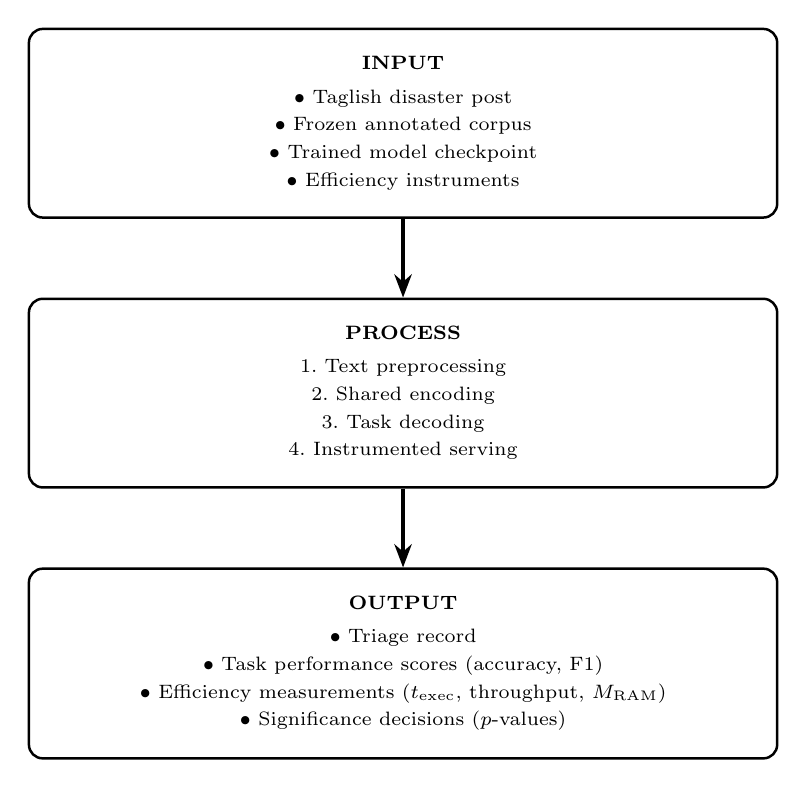
\begin{tikzpicture}[
    font=\small,
    >=Stealth,
    iobox/.style={
        draw=black,
        fill=white,
        rounded corners=5pt,
        align=center,
        inner sep=10pt,
        font=\scriptsize,
        line width=0.9pt,
        text width=8.8cm
    },
    bigarrow/.style={->, very thick, draw=black}
]

    \node[iobox] (input) {
        {\textbf{INPUT}\par}\vspace{4pt}
        $\bullet$~Taglish disaster post\\[2pt]
        $\bullet$~Frozen annotated corpus\\[2pt]
        $\bullet$~Trained model checkpoint\\[2pt]
        $\bullet$~Efficiency instruments
    };

    \node[iobox, below=1.0cm of input] (process) {
        {\textbf{PROCESS}\par}\vspace{4pt}
        1.~Text preprocessing\\[2pt]
        2.~Shared encoding\\[2pt]
        3.~Task decoding\\[2pt]
        4.~Instrumented serving
    };

    \node[iobox, below=1.0cm of process] (output) {
        {\textbf{OUTPUT}\par}\vspace{4pt}
        $\bullet$~Triage record\\[2pt]
        $\bullet$~Task performance scores (accuracy, F1)\\[2pt]
        $\bullet$~Efficiency measurements ($t_{\mathrm{exec}}$, throughput, $M_{\mathrm{RAM}}$)\\[2pt]
        $\bullet$~Significance decisions ($p$-values)
    };

    \draw[bigarrow] (input.south) -- (process.north);
    \draw[bigarrow] (process.south) -- (output.north);

\end{tikzpicture}
\end{document}
